\section{Evaluation: Precision, Recall, F-measure}
\begin{frame}{Mục lục}
	\tableofcontents[currentsection]
\end{frame}

\begin{frame}{Evaluation: Precision, Recall, F-measure}
	Bắt đầu với bài toán \textbf{binary detection}, mục tiêu của bài toán thường phân loại data vào một trong hai class (positive hoặc negative).\\[0.6cm]
	Ví dụ với bài toán kiểm tra tin nhắn spam (spam detection):
	\begin{itemize}
		\item Mục tiêu của bài toán là xác định các tin nhắn được coi là \textbf{spam} (positive) hay \textbf{không spam} (negative).
		\pause
		\item 	Tuy nhiên, để biết biết một tin nhắn có \textbf{thật sự} là spam hay không thì vẫn phải cần con người nhận định.
		\item Những label (spam hoặc không spam) mà do con người nhận định còn được gọi là \textbf{gold labels}.
	\end{itemize}
\end{frame}

\begin{frame}{Evaluation: Precision, Recall, F-measure}
	Để đánh giá các hệ thống cho các bài toán detection như trên, công cụ cơ bản nhất hay sử dụng là \textbf{confusion matrix} (ma trận nhầm lẫn). \\[0.5cm]
	\textbf{Confusion matrix} là một ma trận 2 chiều gồm một chiều là \textbf{gold labels} (Nhãn đúng), và một chiều là \textbf{system output labels} (Nhãn dự đoán của hệ thống).
\end{frame}


\begin{frame}{Evaluation: Precision, Recall, F-measure}
	Xét ví dụ về \textbf{confusion matrix} cho bài toán phân loại nhị phân (binary classfication):
	\begin{figure}
		\centering
		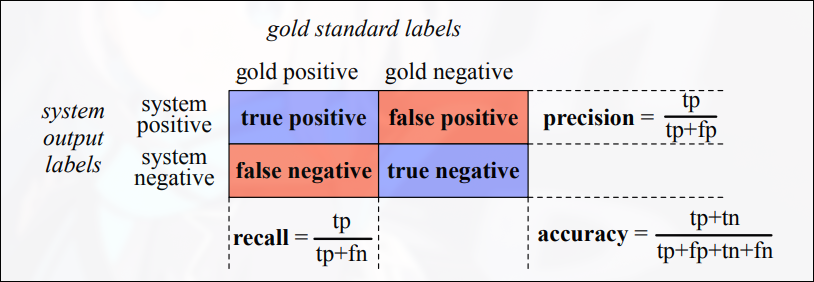
\includegraphics[width=1\linewidth]{confusion_matrix}
	\end{figure}
\end{frame}

\begin{frame}{Evaluation: Precision, Recall, F-measure}
	Một số định nghĩa:
{\small
	\begin{itemize}
		\item \textbf{True positive} (TP): system đoán positive, \textbf{và nó đúng} là positive.
		\item \textbf{False positive} (FP): system đoán positive, \textbf{nhưng nó lại} là negative.
		\item \textbf{False negative} (FN): system đoán negative, \textbf{nhưng nó lại} là positive.
		\item \textbf{True negative} (TN): system đoán negative, \textbf{và nó đúng} là negative.
	\end{itemize}
}
\end{frame}

\begin{frame}{Evaluation: Precision, Recall, F-measure}
	Accuracy là một thước đo cho biết \textbf{tỷ lệ dự đoán đúng} trên \textbf{toàn bộ mẫu dữ liệu}. Công thức của Accuracy:
	\[
	\mathrm{\textbf{Accuracy}}=\frac{\mathrm{TP}+\mathrm{TN}}{\mathrm{TP}+\mathrm{FP}+\mathrm{TN}+\mathrm{FN}}
	\]
	\pause 
	Tuy nhiên, \textbf{Accuracy} không phải lúc nào cũng phản ánh đúng hiệu quả của mô hình. \\[0.1cm]
	Giả sử dữ liệu có 1,000,000 trường hợp negative, nhưng chỉ có 10 trường hợp positive. Nếu system luôn đoán là negative thì accuracy vẫn gần như $100\%$. 
\end{frame}

\begin{frame}{Evaluation: Precision, Recall, F-measure}
	\textbf{Precision} là một thước đo cho biết tỉ lệ mẫu \textbf{thật sự là positive} trên \textbf{toàn bộ mẫu} mà hệ thống \textbf{đoán là positive}:
	\[
	\mathrm{\textbf{Precision}}=\frac{\mathrm{true\ positives}}{\mathrm{true\ positives}+\mathrm{false\ positives}}
	\]
	\pause
	\textbf{Recall} là thước đo cho biết tỉ lệ mẫu mà hệ thống \textbf{đoán đúng} trên tất cả các mẫu \textbf{thật sự là positive}:
	\[
	\text{\textbf{Recall}} = \frac{\mathrm{true\ positives}}{\mathrm{true\ positives} + \mathrm{false\ negatives}}
	\]
\end{frame}

\begin{frame}{Evaluation: Precision, Recall, F-measure}
Bên cạnh Precision và Recall, có nhiều độ đo kết hợp từ hai độ đo trên. Đơn giản nhất là \textbf{F-measure}:
\[
F_{\beta} = \frac{(\beta^2 + 1)PR}{\beta^2 P + R}
\]
Hệ số $\beta$ được dùng để điều chỉnh mức độ đóng góp của precision và recall trong F-measure:
\pause
\begin{itemize}
	\item Nếu $\beta > 1$, recall sẽ được coi trọng hơn precision. 
	\item Nếu $\beta < 1$, precision sẽ được ưu tiên hơn recall.
	\item Khi $\beta = 1$, precision và recall được xem trọng như nhau, nên đây là \textbf{trường hợp cân bằng}.
\end{itemize}

\end{frame}

\begin{frame}{Evaluation: Precision, Recall, F-measure}
Bên cạnh Precision và Recall, có nhiều độ đo kết hợp từ hai độ đo trên. Đơn giản nhất là \textbf{F-measure}:
\[
F_{\beta} = \frac{(\beta^2 + 1)PR}{\beta^2 P + R}
\]
	\textbf{Trường hợp cân bằng} ($\beta = 1$) là trường hợp được sử dụng rộng rãi nhất, còn được gọi là $F_{\beta=1}$ hay $F_1$: 
	\begin{equation}
		F_1 = \frac{2PR}{P + R}
		\tag{4.42}
	\end{equation}
\end{frame}

\begin{frame}{Evaluation: Precision, Recall, F-measure}
	\textbf{F-measure} được tính bằng \textbf{weighted harmonic mean} (trung bình điều hòa có trọng số) giữa precision và recall. \\[0.2cm]
	
	\textbf{Harmonic mean} (trung bình điều hòa) là nghịch đảo của trung bình cộng các số nghịch đảo:
	\begin{equation}
		\mathrm{HarmonicMean}(a_1, a_2, a_3, a_4, \ldots, a_n)
		=
		\frac{n}{
			\frac{1}{a_1} + \frac{1}{a_2} + \frac{1}{a_3} + \cdots + \frac{1}{a_n}
		}
		\tag{4.43}
	\end{equation}
	\pause
	Và do đó, F-meansure được viết thành:
	\begin{equation}
		\begin{alignedat}{2}
			F = \frac{1}{\alpha \frac{1}{P} + (1 - \alpha)\frac{1}{R}}
			\qquad \text{hay} \qquad
			&F = \frac{(\beta^2 + 1)PR}{\beta^2 P + R} \\
			& \text{với } \beta^2 = \frac{1 - \alpha}{\alpha}
		\end{alignedat}
		\tag{4.44}
	\end{equation}
\end{frame}

\begin{frame}{Evaluation: Precision, Recall, F-measure}
	Những ví dụ và độ đo trên được dùng cho các bài toán có 2 class. \\[0.2cm]
	
	Vậy với các bài toán nhiều hơn 2 class thì sao? \\[0.2cm]
	Ví dụ: 
	\begin{itemize}
		\item Sentiment Analysis (Phân tích cảm xúc) gồm 3 class (Positive, Negative, Neutral)
		\item Text classification (Phân loại từ)
		\item $\ldots$
	\end{itemize}
\end{frame}

\begin{frame}{Evaluation: Precision, Recall, F-measure}
	Xét ví dụ bài toán phân loại thành 3 class urgent, normal và spam:
	\begin{figure}
		\centering
		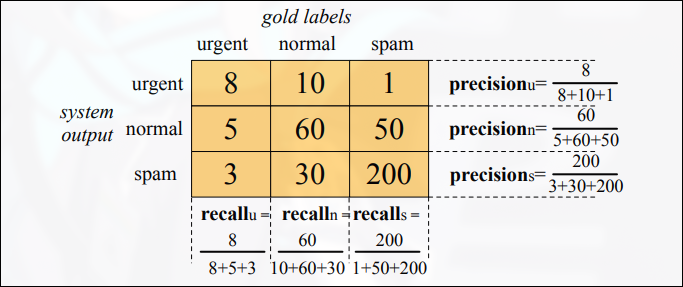
\includegraphics[width=1\linewidth]{confusion_matrix3x3}
	\end{figure}
	
\end{frame}

\begin{frame}{Evaluation: Precision, Recall, F-measure}
	Ta có thể tính precision và recall riêng cho từng class. Nói cách khác, mỗi class sẽ được xem như một bài toán riêng để đo lường hệ thống trên chính class đó.
	
	\begin{figure}
		\centering
		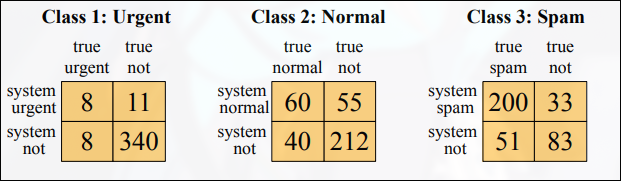
\includegraphics[width=1\linewidth]{confusion_matrix2}
	\end{figure}
	
\end{frame}


\begin{frame}{Evaluation: Precision, Recall, F-measure}
	Tuy nhiên, nếu chỉ nhìn từng class riêng lẻ thì sẽ khó có được một \textbf{kết luận chung} cho toàn bộ hệ thống. Vì vậy, ta cần gộp các giá trị này lại thành một metric tổng quát hơn. \\[0.2cm]
	
	Chúng ta có thể gộp các giá trị này theo 2 cách:
	\begin{itemize}
		\item Với \textbf{Macroaveraging}, ta tính metric riêng cho từng class xong lấy trung bình cộng lại.
		\item Với \textbf{Microaveraging}, ta gộp nhóm các quyết định theo từng class thành một confusion matrix riêng, rồi tính precision và recall chung cho toàn hệ thống.
	\end{itemize}
	
\end{frame}

